\section{Numerical experiments. }

In this section we present the result of the DNS introduced in the previous chapter. 
We recall that we are working with a set of simulations covering the parameters ranges display in \ref{tab:simulations_recall}. 
\begin{table}[h!]
    \centering
    \caption{Dimensionless parameter range investigated in this work.}
    \begin{tabular}{|ccccccc|ccc|}
        \hline
        \multicolumn{7}{|c}{Primary parameters} & \multicolumn{3}{||c|}{Secondary parameters}\\ \hline
        \multicolumn{1}{|c|}{$Ga$}                               & \multicolumn{1}{c|}{$Bo$}                   & \multicolumn{1}{c|}{$\phi$} & \multicolumn{1}{c|}{$\lambda$}                    & \multicolumn{1}{c|}{$\zeta$}                & \multicolumn{1}{c|}{$N_b$} & $t^*_\text{end}$ & \multicolumn{1}{||c|}{$\mathcal{L}/d$} & \multicolumn{1}{c|}{$Re$}  & $We$   \\ \hline
        \multicolumn{1}{|c|}{\multirow{4}{*}{$5\rightarrow 80$}} & \multicolumn{1}{c|}{\multirow{4}{*}{$0.5$}} & \multicolumn{1}{c|}{$1\%$}  & \multicolumn{1}{c|}{\multirow{4}{*}{$10$ \& $1$}} & \multicolumn{1}{c|}{\multirow{4}{*}{$0.9$}} & \multicolumn{1}{c|}{$160$} & $400$           & \multicolumn{1}{||c|}{$20$}            & \multicolumn{1}{c|}{$1.1\to 110$} & {$0.03\to 0.95$} \\ 
        \multicolumn{1}{|c|}{}                                   & \multicolumn{1}{c|}{}                       & \multicolumn{1}{c|}{$5\%$}  & \multicolumn{1}{c|}{}                             & \multicolumn{1}{c|}{}                       & \multicolumn{1}{c|}{$800$} & $400$           & \multicolumn{1}{||c|}{$20$}            & \multicolumn{1}{c|}{$0.8\to 92$} &  {$0.02\to 0.67$}\\ 
        \multicolumn{1}{|c|}{}                                   & \multicolumn{1}{c|}{}                       & \multicolumn{1}{c|}{$10\%$} & \multicolumn{1}{c|}{}                             & \multicolumn{1}{c|}{}                       & \multicolumn{1}{c|}{$200$} & $1000$           & \multicolumn{1}{||c|}{$10$}            & \multicolumn{1}{c|}{$0.64\to 77$}&  {$0.01\to 0.47$}\\ 
        \multicolumn{1}{|c|}{}                                   & \multicolumn{1}{c|}{}                       & \multicolumn{1}{c|}{$20\%$} & \multicolumn{1}{c|}{}                             & \multicolumn{1}{c|}{}                       & \multicolumn{1}{c|}{$400$} & $1000$           & \multicolumn{1}{||c|}{$10$}            & \multicolumn{1}{c|}{$0.43\to 62$}&  {$9\cdot 10^{-3}\to 0.31$}\\ \hline
        \end{tabular}
    \label{tab:simulations_recall}
\end{table}
In a first step we are seeking for a validation of the theoretical results with the DNS. 
Thus, we will make use of the DNS at $Ga = 5$ which are considered to be comparable to the Stokes regime used for the theory. 
However, note that at $Ga = 5$, $Re \approx 1$ consequently inertial effects are actually already present. 
Nevertheless, due to numerical constraint lower \textit{Reynolds} numbers could not be reached. 

The two main results that we are seeking to validate are, the disturbance fields expression \eqref{eq:v_nst_solution_adim} and the \textit{Reynolds} stress closure tensor, \eqref{eq:functional_form_avg}. 
Consequently, in the first part of this section we focus on the comparison of $\textbf{v}_f^\text{nst}$ obtained with the DNS to the solution given by \ref{eq:v_nst_solution_adim}.
Then, we compare the numerical value of $\avg{\chi_f \textbf{u}_f'\textbf{u}_f'}$ with the prediction of \ref{eq:functional_form_avg}. 
And finally, we try to extend \ref{eq:functional_form_avg} to non-negligible inertial effect, i.e. for higher $Re$. 

\subsection{The nearest neighbors conditionally averaged disturbance velocity field}

In order to reconstruct $\textbf{v}_f^\text{nst}$ with the DNS we must discretize \ref{eq:def_f_nst}. 
We proceed as follows: 
(1) We consider all simulations time step and location in the mesh as an independent configuration $\FF$. 
(2) Thus we consider that $\textbf{u}_f^0[\textbf{x},\FF,t]$ is given by any $\textbf{u}[c,t]$ where $c$ is the label of a given cell in the mesh and $t$ the time step of the simulation. 
It must be understood that $\FF$ corresponds to all combination of $c$ and $t$. 
(2) Finally, we discretize the distance $\textbf{r}$ from a point in the mesh to the center of mass of a nearest neighbor in $n^{th}$ intervals, with centering value of $\textbf{r}_k$ of $\textbf{r}_k = 1,\ldots,n$. 
Under this hypothesis, the \textit{nearest neighbors conditionally averaged} velocity fields, $\textbf{u}_f^\text{nst}$, can be obtained numerically as, 
\begin{equation}
    \textbf{u}_f^\text{nst}(\textbf{r}_k)
    = 
    \frac{1}{E_k}
    \sum_{\FF_k}^{E_k}
    \sum_i^N
    \textbf{u}[c,t] h_i[c,t]
    \label{eq:vnst_DNS}
\end{equation}
where $E_k$ corresponds to the total number of events and $N$ to the total number of particle in the flow.
$h_i[c,t]$ corresponds to the function $h_i[\textbf{x},t,\FF]$ defined with \ref{eq:h_i_def} evaluated at time step $t$ and at the center of cell $c$. 
Thus, $h_i[c,t] = 1$ when teh $i^{th}$ droplet is the nearest neighbor to the location of the cell center $c$. 
This function depends on course of the center of mass of the droplets, which are obtained using the same approach as in the previous chapters.
Then, to recover $\textbf{v}_f^\text{nst}/U$ from $\textbf{u}_f^\text{nst}$, we simply measure the mean relative phase velocity $U$ within the DNS, and use the formula: $\textbf{v}_f^\text{nst} /  U = \textbf{u}_f^\text{nst} / U -1 $. 



In \ref{fig:vnst_DNS} we display the reconstructed the velocity fields based on the DNS, according to \ref{eq:vnst_DNS}. 
Because, our DNS results of rising droplets form a homogeneous emulsion rising in the direction of buoyancy, our results are to be compared with the theoretical prediction displayed on \ref{fig:vnst_vertical}. 
\begin{figure}
    \centering
    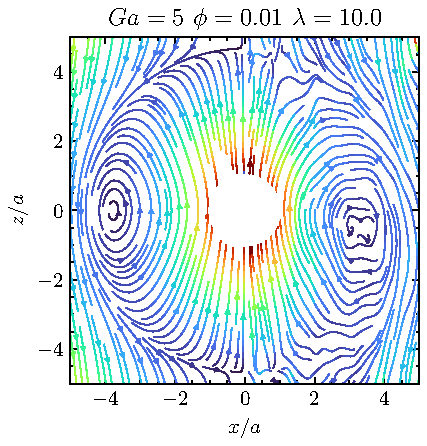
\includegraphics[width = 0.32\textwidth]{image/HOMOGENEOUS_final/Stream/Stream_PHI_1_Ga_5_l_10.pdf}
    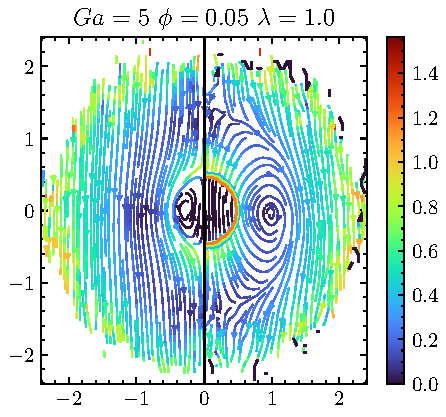
\includegraphics[width = 0.32\textwidth]{image/HOMOGENEOUS_final/Stream/Stream_PHI_5_Ga_5_l_10.pdf}
    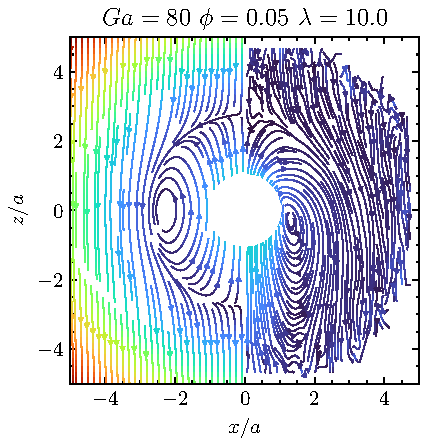
\includegraphics[width = 0.32\textwidth]{image/HOMOGENEOUS_final/Stream/Stream_PHI_5_Ga_80_l_10.pdf}
    \caption{Streamlines of the disturbance velocity field $\textbf{v}^\text{nst}$, in the cross-section given by the plane $(\textbf{e}_x,\textbf{e}_z)$, for two volume fractions $\phi = 0.01$ (left) and $\phi = 0.05$ (middle) at $\lambda = 10$ and $Ga = 5$.
    (right) plot of the inertial case $Ga = 80$. 
    The left side of the panel ($x/a < 0$), we have re-plotted the theoretical solution provided by \ref{eq:v_nst_solution_adim}.   
    The right side of the panel ($x/a > 0$), we have reconstructed the streamlines obtained with the DNS, using \ref{eq:vnst_DNS}. 
    The color map indicates the magnitude of the velocity, from black which corresponds to a velocity magnitude of 0, to the color at the interface of the droplet which corresponds to a magnitude of 1.}
    \label{fig:vnst_DNS}
\end{figure}
The common points that shears the velocity fields from \ref{eq:vnst_DNS} to the one displayed in \ref{eq:vnst_vertical} are the following: 
(1) both exhibit approximately the same wake close to the interface of the droplet. 
That is the wake of an isolated rising vertical droplet. 
(2) For a distance large enough  from the droplets center we see appear the downstream flows, which is generated due to buoyancy forces. 
(3) The confinement zone, delimited by the null normal velocity, follows the same trends as the theoretical prediction, i.e. the radius is smaller for higher $\phi$. 
Additionally, the radius of the confinement zone have approximately the same size for both cases. 

Regarding the differences, we can notice that for the case $\phi = 0.01$, displayed on \ref{fig:vnst_DNS} (middle) the wake of the particle is slightly asymmetric, while the theoretical solution is purely symmetric. 
The fore-aft symmetry of the wake of a particle as displayed in \ref{fig:vnst_vertical} is typically due to the absence of inertial effect. 
Thus, the non fore-aft symmetry observed on the plot, \ref{fig:vnst_DNS} (right), is due to the non-negligible inertial effect present for this case. 
Indeed, as reported in \ref{tab:simulations_recall} the \textit{Reynolds} number for this case is $Re \approx 1$, implying that the inertial effects cannot be neglected. 
In opposition at $\phi = 0.05$ the numerical results exhibit a nearly fore-aft symmetric wake. 
Which is consistent with the previous remark since for this case $Re < 1$. 

To extends our understanding we have also display on \ref{eq:vnst_DNS} (right) a high inertial case, with  $Ga = 80$. 
In this case we clearly see that the wake exhibit fore-aft asymmetry, which confirm that this trends comes with inertial effects. 
Additionally, we can notice that the top boundary corresponding to the confinement zone is approximately at the same location as the theoretical prediction. 
However, the downstream boundary is clearly different from the one predicted by the theoretical prediction, again that is because the fore-aft symmetry of the flow is broken.  

Although, the effect of inertial generate a for-aft asymmetry, it will not necessarily impact the velocity variance. 
Indeed, the variance is independent of the asymmetric behavior of the distribution. 
Absolutely, the asymmetry is measured by the triple velocity correlation $\avg{\chi_f\textbf{u}_f'\cdot \textbf{u}_f' \textbf{u}_f'}$ appearing in the pseudo turbulent energy equation, not by the \textit{Reynolds} stress. 
However, this is out the scope of the present work. 



% \begin{figure}
%     \centering
%     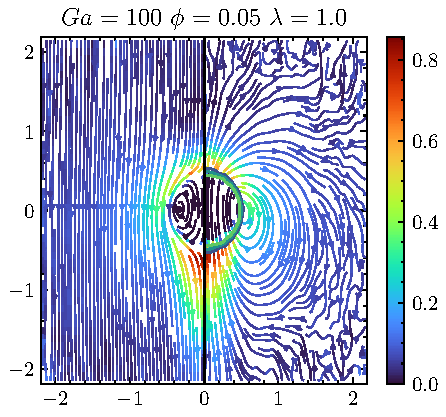
\includegraphics[width = 0.33\textwidth]{image/HOMOGENEOUS_NEW/Stream/Stream_PHI_5_Ga_100_l_10.pdf}
%     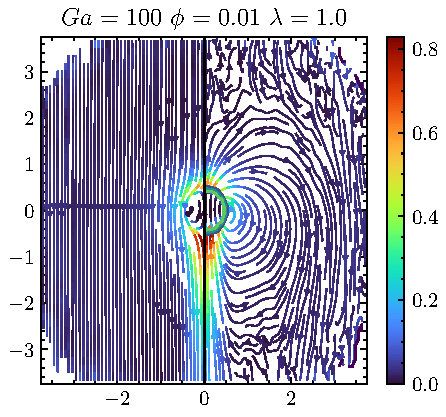
\includegraphics[width = 0.33\textwidth]{image/HOMOGENEOUS_NEW/Stream/Stream_PHI_1_Ga_100_l_10.pdf}
%     \caption{Streamlines of the disturbance velocity field $\textbf{v}^\text{nst}(\textbf{r}_f)$  reconstructed from the DNS, in the cross-section given by the plane $(\textbf{e}_x,\textbf{e}_z)$, for two volume fraction $\phi = 0, 0.01$ and $0.05$ at $\lambda = 10$.  
%     The color map indicates the magnitude of the velocity, from black which corresponds to a velocity magnitude of 0, to red which corresponds to the maximum velocity at the droplet boundary.}
%     \label{fig:vnst_DNS}
% \end{figure}

\subsection{Vertical velocity variance}

As discussed in the previous section, in the situation reproduced by the DNS, the velocity variance is given by \ref{eq:functional_form_avg} without the contribution of gravity (see \eqref{eq:cancelation1} and \ref{eq:cancelation2}). 
Additionally, at $Re \approx 1$ we assert that the particle vertical velocity variance $\pavg{\textbf{u}_\alpha'\textbf{u}_\alpha'}_{yy}$ is negligible. 
In the next subsection we show that this assumption will be shown to be invalid for the horizontal velocity variance. 
Under these conditions, the vertical component of the velocity variance given by \ref{eq:functional_form_avg} is expressed by the following formula, 
\begin{equation}
    \frac{\avg{\chi_f \textbf{u}_f'\textbf{u}_f'}_{zz}}{U^2}
    = \phi^{2/3} \left(
        \frac{2}{3}C_e^{(1)}+ C_e^{(2)}
    \right)
    = 
    \phi^{2/3}\Gamma\left(\frac{1}{3}\right) \frac{7}{60}\frac{(2+3\lambda)^2 }{(\lambda+1)^2}
    % \left(e^{-Re} - 1 \right)/2
    + \mathcal{O}(\phi) 
    % . 
    \label{eq:theoritical_simplified}
\end{equation}


\subsubsection{Statistics computations within DNS}

Following \citet{du2022analysis} we consider ergodicity at all time of the numerical experiment.
Thus, the ensemble average of a quantity $X$ can be approximated by a spatial average $\Xavg{X}$ and a time average $\Tavg{X}$ such that $\int X d\PP = \avg{X} \approx \Xavg{\Tavg{X}} = \Tavg{\Xavg{X}}$.
Consequently, the ensemble average of a numerical field, $X$, is taken through space and time such that,
\begin{equation}
    \avg{X}
    = \Tavg{\Xavg{X}}
    = \frac{1}{ t_{end} - t_0}\int_{t_0}^{t_{end}} 
    \Xavg{X}(t) dt
\end{equation}
where, 
\begin{equation}
    \Xavg{X}(t)
    = \frac{1}{L^3}\int 
    X(\textbf{x},t) d\textbf{x}
\end{equation}
where $L$ is the length of the cubic domain.
$t_0$ and $t_{end}$ is the starting time of sampling and the time duration of the simulation, respectively.
In practice, we take $t_0$ such that the simulation reach a statistically steady regime for $t>t_0$.  
Both $t_{end} $ and $t_0$ are given in \ref{ap:A} after several validations studies. 

Therefore, to compute the phase average of the local phase velocity $\textbf{u}_k^0$, we simply perform an integration over space and time, 
\begin{equation*}
    \textbf{u}_k = \frac{1}{\phi_k} \Tavg{\Xavg{\chi_k \textbf{u}_k^0}}
\end{equation*}
To compute continuous phase averaged quantities such as \ref{eq:def_uuc} it is a little more complicated, we obtain
\begin{equation}
    \avg{\chi_f\textbf{u}_f' \textbf{u}_f'}
    % = \Tavg{\Xavg{\chi_f \textbf{u}_f' \textbf{u}_f'}}
    = \Tavg{\Xavg{\chi_f (\textbf{u}_f^0 -\textbf{u}_f ) (\textbf{u}_f^0 -\textbf{u}_f)}}
    = \Tavg{\Xavg{\chi_f \textbf{u}_f^0 \textbf{u}_f^0}}
    -  \phi_f  \textbf{u}_f \textbf{u}_f.
    \label{eq:def_uuf_num} 
\end{equation}
where the indicator funciton $\chi_f$ must be understood as its approximation in the DNS, i.e the color function $1 - \alpha_d$. 
Consequently, \ref{eq:def_uuc_num} indicate that we must take the average of the product of the velocities, and then we retrieve the mean velocities' product.  



\subsubsection{Comparison with the DNS}
In \ref{fig:uuyy} (right) we compared \ref{eq:theoritical_simplified} to the numerical result.
At low volume fraction and for all $\lambda$ very good agreements are obtained. 
As expected as $\phi$ increase, the gap between the value predicted by \ref{eq:theoritical_simplified} and the DNS becomes larger.
Specifically, the theoretical value tends to overestimate the velocity variance.   
Interestingly at $\lambda = 10$ \ref{eq:theoritical_simplified} seems to predict a good estimation for the Reynolds stress regardless of the volume fraction $\phi$. 
However, since no interaction terms of any kind were considered in the theory, this good agreement is likely coincidental.
\begin{figure}
    \centering
    % 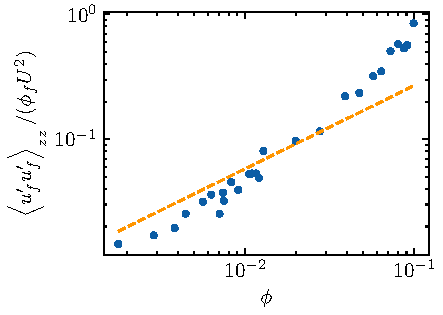
\includegraphics[height = 0.25\textwidth]{image/HOMOGENEOUS_final/CA/cartellier.pdf}
    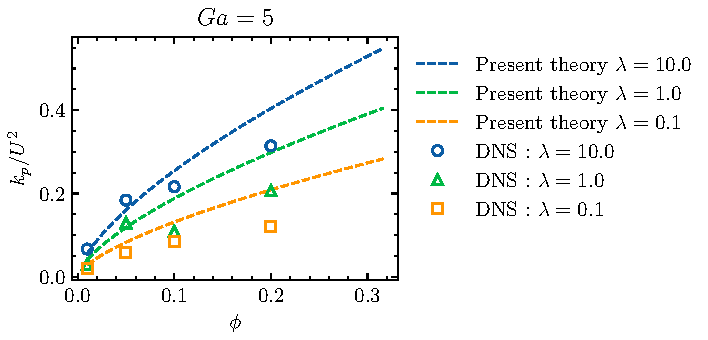
\includegraphics[height = 0.25\textwidth]{image/HOMOGENEOUS_final/CA/UUyy_Ga_5.pdf}
    \caption{Dimensionless value of the vertical velocity variance  in terms of the volume fraction $\phi$ for various $\lambda$ in the low inertial regime ($Ga = 5$). 
    % (left) Experimental  results  of \citet{cartellier2009induced} compared to \ref{eq:theoritical_simplified} with $\lambda = 0$ (dash dotted line) original scaling of \citet{cartellier2009induced}. 
    Comparison of the ``Present theory'' \eqref{eq:theoritical_simplified} against the velocity variance obtained with DNS results according to \eqref{eq:def_uuf_num}. 
    }
    \label{fig:uuyy}
\end{figure}
The red-dashed line in \ref{fig:uuyy} (right) represents the potential flow solution of \citet{van1998pseudo} given by \ref{eq:van_wingarden_sol}. 
As a matter of fact, this model underpredicts largely the magnitude of the vertical pseudo-turbulence.



\subsubsection{Comparison with the literature}

In \ref{fig:uuyy2} (left) we compare our results to the  experimental measurement of \citet{cartellier2009induced}. 
Again, we observe reasonable agreements from $\phi = 10^{-3}$ to moderate volume fraction ($\phi \approx 0.03$). 
In the low volume fraction regime \citet{cartellier2009induced} found that $\avg{\chi_f\textbf{u}_f'\textbf{u}_f'} / U^2 \sim \phi^{0.7 \pm 0.03}$,  while \ref{eq:theoritical_simplified} with $\lambda = 0$ predicts, $\avg{\chi_f\textbf{u}_f'\textbf{u}_f'} / U^2 \sim 1.25017 \cdot \phi^{2/3} $. 
Thus, our results overestimate \citet{cartellier2009induced} best fits by $25\%$. 
This can be explained by the non-negligible inertial effects present in \citet{cartellier2009induced} experiments, indeed they measured a $Re \approx 10$. 
\begin{figure}
    \centering
    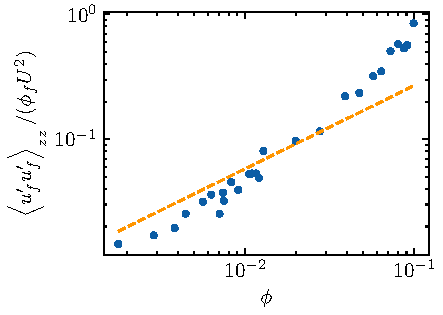
\includegraphics[height = 0.25\textwidth]{image/HOMOGENEOUS_final/CA/cartellier.pdf}
    \caption{Dimensionless value of the vertical velocity variance  in terms of the volume fraction $\phi$ for various $\lambda$ in the low inertial regime ($Ga = 5$). 
    (dots) Experimental  results  of \citet{cartellier2009induced}.
    (dashed line) Theoretical formula \ref{eq:theoritical_simplified} with $\lambda = 0$.
    (dash dotted line) \citet{cartellier2009induced}'s original scaling. 
    }
    \label{fig:uuyy2}
\end{figure}

Considering the good agreements obtained with both, the numerical results and \citet{cartellier2009induced} experiments, we can state that \ref{eq:theoritical_simplified} is validated. 
Indeed, it is reasonable to assume that the slight disparities observed between these results and the theory is due to the inertial effects or a non-negligible volume fraction. 

\subsection{The Horizontal velocity variance}

Using the general formulation \ref{eq:functional_form_avg}, we write the horizontal component of the \textit{Reynolds} as, 
\begin{equation}
    \frac{\avg{\chi_f \textbf{u}_f'\textbf{u}_f'}}{U^2}
    = \phi^{2/3}\Gamma\left(\frac{1}{3}\right) \frac{1}{240}\frac{(2+3\lambda)^2 }{(\lambda+1)^2}
    + 
    C^{(1)}_e \left[
    \frac{\pavg{\textbf{u}_\alpha'\textbf{u}_\alpha'}_{xx}}{n_p U^2}
    - \frac{2k_p}{3U^2}  
    \right]
    + C^{(2)}_e
    \frac{2k_p}{U^2}  
    \label{eq:Horizontal_varience}
\end{equation}
Notice how the first term on the right-hand side of \ref{eq:Horizontal_varience} is smaller than the one provided by \ref{eq:theoritical_simplified}. 
This means that the horizontal velocity variance produced by the mean vertical motion of the droplets is significantly lower than the vertical velocity variance. 
Additionally, in this formulation we have kept the terms related to the particle center of mass velocity variance. 
The reason for this choice will be clarified latter. 
% Thus, in this situation we might expect that the particle center of mass velocity variance is non-negligible, compared to the first contribution of \ref{eq:Horizontal_varience}. 


In \ref{fig:uuxx} (right) we display the numerical values of the horizontal velocity variance against the theoretical results provided by, \ref{eq:Horizontal_varience}. 
\begin{figure}
    \centering
    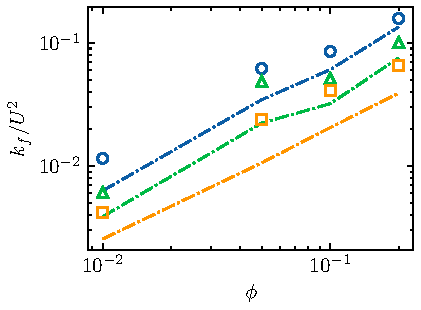
\includegraphics[height = 0.25\textwidth]{image/HOMOGENEOUS_final/CA/UUxx2_Ga_5.pdf}
    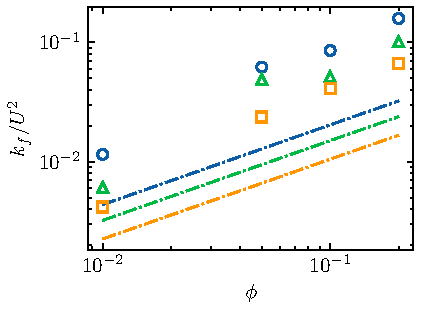
\includegraphics[height = 0.25\textwidth]{image/HOMOGENEOUS_final/CA/UUxx_Ga_5.pdf}
    \caption{Dimensionless value of the horizontal velocity varience  in terms of the volume fraction $\phi$ for various $\lambda$ in the low inertial regime ($Ga = 5$). 
    (left) Theoretical results \eqref{eq:Horizontal_varience} \underline{with} the particle velocity variance included
    (right) Theoretical results  \eqref{eq:Horizontal_varience} \underline{without} the particle velocity variance included. 
    }
    \label{fig:uuxx}
\end{figure}
It is seen that for all $\phi$ and $\lambda$ the theoretical predictions given by \ref{eq:Horizontal_varience}, when neglecting the particle phase velocity, i.e.  $k_p =0$ and $ \pavg{\textbf{u}_\alpha'\textbf{u}_\alpha'}_{xx} = 0 $, is underestimating the particle phase velocity. 
Since, the velocity variance produced by a Stokes disturbance fields will be alway larger (in dimenisonless form) than the disturbance field given by an inertial partilce, we must conclude that the lake of velocity varience predicted by the theortry is due to the non-inclusion of the particle phase velocity. 
In other word, the effect of inertia is to lower the dimensionless \textit{Reynolds} stress, thus if we underpredict it it must comes from other reason than inertia. 
According to \ref{fig:vnst_DNS} it seems that we rather well predict the effect of confinement, i.e. the effect of the volume fraction, at $Ga = 5$.
Thus, the only reason why the fluid phase velocity variance is underestimated is because of the neglected particle phase velocity variance.  

On \ref{fig:uuxx} (left) we display the numerical values of the horizontal velocity variance against the theoretical results provided by, \ref{eq:Horizontal_varience}, including the values of $k_p$ and $\pavg{\textbf{u}_\alpha'\textbf{u}_\alpha'}_{xx}$ that are obtained numerically. 
The prediction in the dense regime ($\phi = 0.2$) seem greatly improved. 
In the dilute regime we still obtain a significant error of about $20\%$. 
At this stage it is hard to explain where does these differences come from. 

We conclude that due to the relatively low magnitude of the horizontal velocity variance of the average wake of particles, the particle phase variance can no longer be neglected and must be accounted for. 
Furthermore, when developing an algebraic model for the \textit{Pseudo-turbulent} tensor, it is essential to consider the impact of the particle phase velocity variance. 
In other words, a closure model for the particle phase velocity variance should be constructed first and incorporated into the \textit{Reynolds stress} model as outlined in \ref{eq:functional_form_avg}. 


\subsection{Extension to higher inertial effects. }

In this subsection we extend our model to higher inertial number $Re$. 
We assume the following properties for the creation of our semi-empirical model: 
(1) In the low inertial regime ($Re=0$) and low volume fraction ($\phi=0$) the \textit{Reynolds stress} must be given by the expression \ref{eq:functional_form_avg}. 
(2) The functional form given by \ref{eq:functional_form_avg} is preserved at finite $Re$. 
Meaning that the scalar $C_e^{(1)}$ and $C_e^{(2)}$ are the only allowed degree of freedom. 
(3) The empirical fit of the constant  $C_e^{(1)}$ and $C_e^{(2)}$ should not take in account the effect of the particle phase velocity fluctuation, since these are already taken in account through the terms $\pavg{\textbf{u}_\alpha'\textbf{u}_\alpha'}$ and $k_p$ in \ref{eq:functional_form_avg}. 
This, means that we must perform the fit on the numerical data while including the particle velocity fluctuation obtained in our DNS in the formula \eqref{eq:functional_form_avg}.
That way $C_e^{(1)}$ and $C_e^{(2)}$ will represent only the modification of the pseudo turbulence due to the averaged wakes.  

According to \ref{eq:functional_form_avg} the pseudoturbulence kinetic energy of the fluid at $Re = 0$ is given by,
\begin{equation}
    k_f^{Re = 0}
    = 
    C_e^{(0)}  \left(\frac{1}{2}  + 3 k_p^*\right)  
\end{equation}
\begin{equation}
    k_f
    = 
    k_f^{Re = 0}
    \cdot \frac{\left(e^{-Re} +1\right)}{2}
    \label{eq:semi_empirical}
\end{equation}
As shown in \ref{fig:kf}

\tb{inertial effect of sedimenting susp + tennet }
\begin{figure}
    \centering
    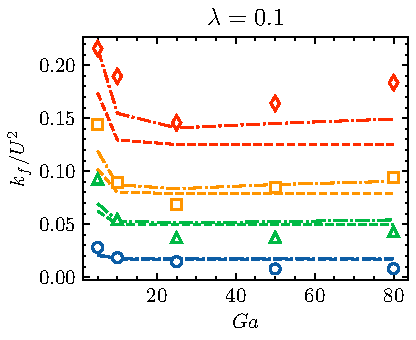
\includegraphics[height = 0.25\textwidth]{image/HOMOGENEOUS_final/CA/KF2_l_0.pdf}
    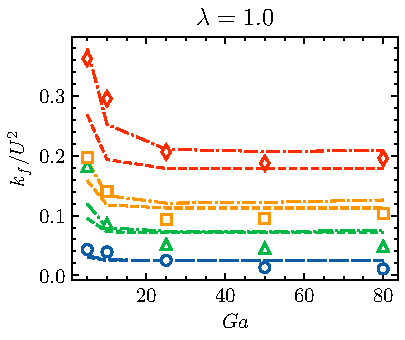
\includegraphics[height = 0.25\textwidth]{image/HOMOGENEOUS_final/CA/KF2_l_1.pdf}
    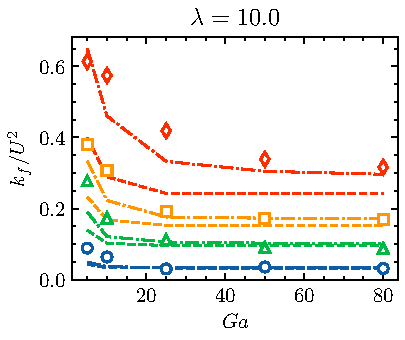
\includegraphics[height = 0.25\textwidth]{image/HOMOGENEOUS_final/CA/KF2_l_10.pdf}
    \caption{Dimensionless continuous phase pseudo turbulent energy, $k_f/U^2$ in terms of the \textit{Galileo} number.
    (left) $\lambda = 0.1$
    (middle) $\lambda = 1$
    (right) $\lambda = 10$
    (Symbols) DNS results computed according to \ref{eq:def_uuf_num}
    ($\pmb\bigcirc$) $\phi = 0.01$; ($\pmb\triangle$) $ \phi = 0.05$; ($\pmb\square$) $\phi = 0.1$ ($\pmb\lozenge$) $\phi = 0.2$.
    (dot dashed lines) Semi-empirical formula \ref{eq:semi_empirical} \underline{including} the results of the DNS for the particle phase velocity fluctuations. 
    (dashed lines) Semi-empirical formula \ref{eq:semi_empirical} \underline{excluding} the particle phase velocity fluctuations. 
    }
    \label{fig:kf}
\end{figure}


Regarding the deviatoric part of the tensor it is actually accounted through the constant $b_f = \frac{27}{10}$ in the expression: $C_e^{(1)} = b_f C_e^{(2)}$ \ref{eq:constants}. 
Following, \citet{mehrabadi2015pseudo} we remark on \ref{fig:bf} that this constant is microstructure dependents. 
We choose, 
\begin{equation*}
    b_k = \frac{27}{10}  \text{exp}\left\{- 3\left(\phi^{5/6} + \frac{10^{-3}}{\lambda+1}Re\right)\right\}
\end{equation*}

\begin{figure}
    \centering
    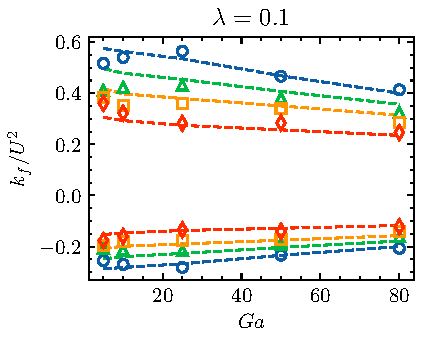
\includegraphics[height = 0.25\textwidth]{image/HOMOGENEOUS_final/CA/D2_l_0.pdf}
    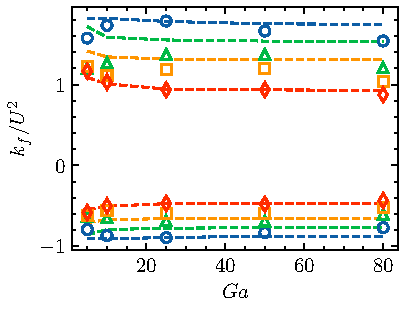
\includegraphics[height = 0.25\textwidth]{image/HOMOGENEOUS_final/CA/D2_l_1.pdf}
    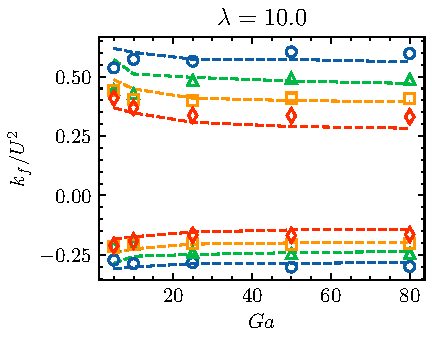
\includegraphics[height = 0.25\textwidth]{image/HOMOGENEOUS_final/CA/D2_l_10.pdf}
    \caption{Deviatoric \textit{Reynolds stress} tensor $\textbf{D}_f$, in terms of the \textit{Galileo} number for multiple viscosity ratios:
    (left) $\lambda = 0.1$,
    (middle) $\lambda = 1$,
    (right) $\lambda = 10$. 
    (Symbols) DNS results computed according to \ref{eq:def_uuf_num}
    ($\pmb\bigcirc$) $\phi = 0.01$; ($\pmb\triangle$) $ \phi = 0.05$; ($\pmb\square$) $\phi = 0.1$ ($\pmb\lozenge$) $\phi = 0.2$.
    (dot dashed lines) Semi-empirical formula \ref{eq:} \underline{including} the results of the DNS for the particle phase velocity fluctuations. 
    (dashed lines) Semi-empirical formula \ref{eq:} \underline{excluding} the particle phase velocity fluctuations. 
    }
    \label{fig:bf}
\end{figure}







\subsection{Final validation}


\begin{figure}
    \centering
    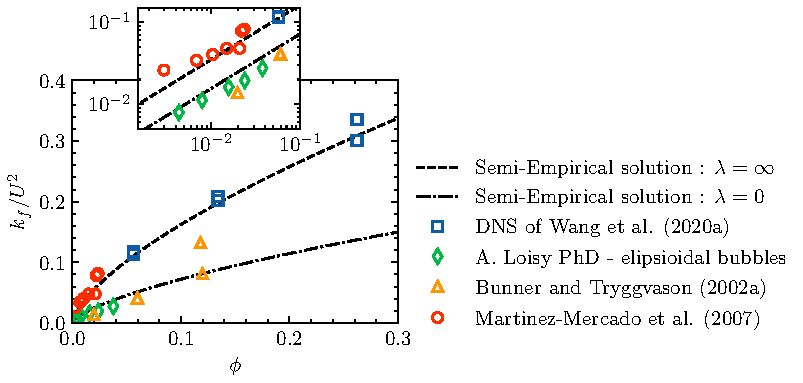
\includegraphics[height = 0.35\textwidth]{image/HOMOGENEOUS_final/CA/KFliterature.pdf}
    \caption{Dimensionless continuous phase pseudo turbulent energy, $k_f/U^2$ in terms of the \textit{Galileo} number.
    (Symbols) DNS and experimental results of: 
    ($\pmb\square$)  Particle-resolved Direct Numerical Simulations (PR-DNS)
    of fixed solid spherical particle assemblies at $20< Re < 100$  by \citet{wang2021numerical}; 
    ($\pmb\lozenge$) Direct numerical simulation (DNS) of rising deformable bubbles at $Re \approx 30$ \citep{loisy2016direct}
    ($\pmb\triangle$) DNS of rising spherical bubbles by \citet{bunner2002dynamics}. 
    ($\pmb\bigcirc$) Experiment of rising spherical bubbles in water by \citet{martinez2007measurement} at $Re \approx 30$. 
    (dot dashed lines) Semi-empirical formula \ref{eq:} at $Re \approx 30$ with $\lambda = 0$. 
    (dashed lines)  Semi-empirical formula \ref{eq:} at $Re \approx 30$ with $\lambda = \infty$.
    }
    \label{fig:trygvason}
\end{figure}
\begin{figure}
    \centering
    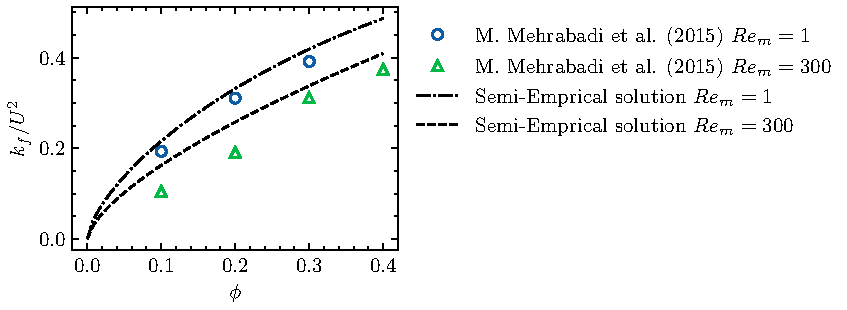
\includegraphics[height = 0.25\textwidth]{image/HOMOGENEOUS_final/CA/tenneti.pdf}
    \caption{Dimensionless continuous phase pseudo turbulent energy, $k_f/U^2$ in terms of the volume fraction $\phi$.
    (Symbols) 
    results of Particle-resolved Direct Numerical Simulations
    of fixed particle assemblies by \citet{mehrabadi2015pseudo}
    ($\pmb\bigcirc$) $Re_m = (1-\phi) \approx 1$; ($\pmb\triangle$) $Re_m \approx 300$;
    (dot dashed lines) Semi-empirical formula \ref{eq:} at $Re_m = 1$
    (dashed lines) Semi-empirical formula \ref{eq:} at $Re_m= = 300$
    }
    \label{fig:tennet}
\end{figure}
\begin{figure}
    \centering
    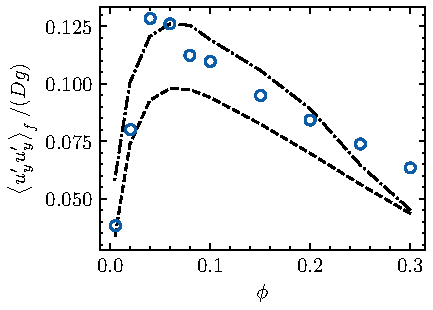
\includegraphics[height = 0.25\textwidth]{image/HOMOGENEOUS_final/CA/tariq.pdf}
    \caption{Dimensionless vertical velocity varience, in terms of the volume fraction $\phi$. 
    (Symbols) results of Particle-resolved Direct Numerical Simulations  of gravitational settling of monodisperse solid spheres by \citet{shajahan2023inertial}. 
    (dot dashed lines) Semi-empirical formula \ref{eq:} \underline{including} \citet{shajahan2023inertial}'s results for the particle phase velocity fluctuations. 
    (dashed lines) Semi-empirical formula \ref{eq:} \underline{excluding} the particle phase velocity fluctuations. 
    }
    \label{fig:tariq}
\end{figure}
